%% LyX 2.0.3 created this file.  For more info, see http://www.lyx.org/.
%% Do not edit unless you really know what you are doing.
\documentclass[english]{article}
\usepackage[T1]{fontenc}
\usepackage[utf8]{luainputenc}
\usepackage{amsmath}
\usepackage{graphicx}

\makeatletter

%%%%%%%%%%%%%%%%%%%%%%%%%%%%%% LyX specific LaTeX commands.
%% Because html converters don't know tabularnewline
\providecommand{\tabularnewline}{\\}

\makeatother

\usepackage{babel}
\begin{document}

\part*{1.Likelihood Function}

L($\gamma$|Data)=P(Data|$\gamma$)=$\underset{n}{\prod}$p($\epsilon_{s-n}$){*}p($\phi_{s-n}$){*}$\frac{d\epsilon_{s}d\phi_{s}}{d\epsilon d\phi}$
.Since the universe is isotropic ,p($\phi_{s}$)=1,and p($\epsilon_{s}$)
is known. In the code I set the distribution of true ellipticity p($\epsilon_{s}$)
to be $\epsilon_{s}(1-\epsilon_{s})$ . It satisfies p(0)=p(1)=0.


\part*{2.Toy data production}

I use the function rand() in C language to produce random datas that
satisfy p($\epsilon_{s}$) and $p(\phi_{s})$. These data are used
as true ellipticity and orientation of galaxies in the code.

Then I use the formulor $\epsilon e^{2i\phi}=\epsilon_{s}e^{2i\phi_{s}}+\gamma.$
To shear the unlensed $\epsilon_{s}$,$\phi_{s}$ to lensed $\epsilon$and
$\phi$.


\part*{3.Likelihood function Calculation}

For any $\gamma$ on the complex plane we can recover unlensed $\epsilon_{s}$and
$\phi_{s}$,and calculate its likelihood.Since the likelihood is very
small when the number of data sample N is large,the code uses Log(likelihood).

the ($\gamma-\gamma_{true}$)-likelihood contour picture is showed
below with N=1000.

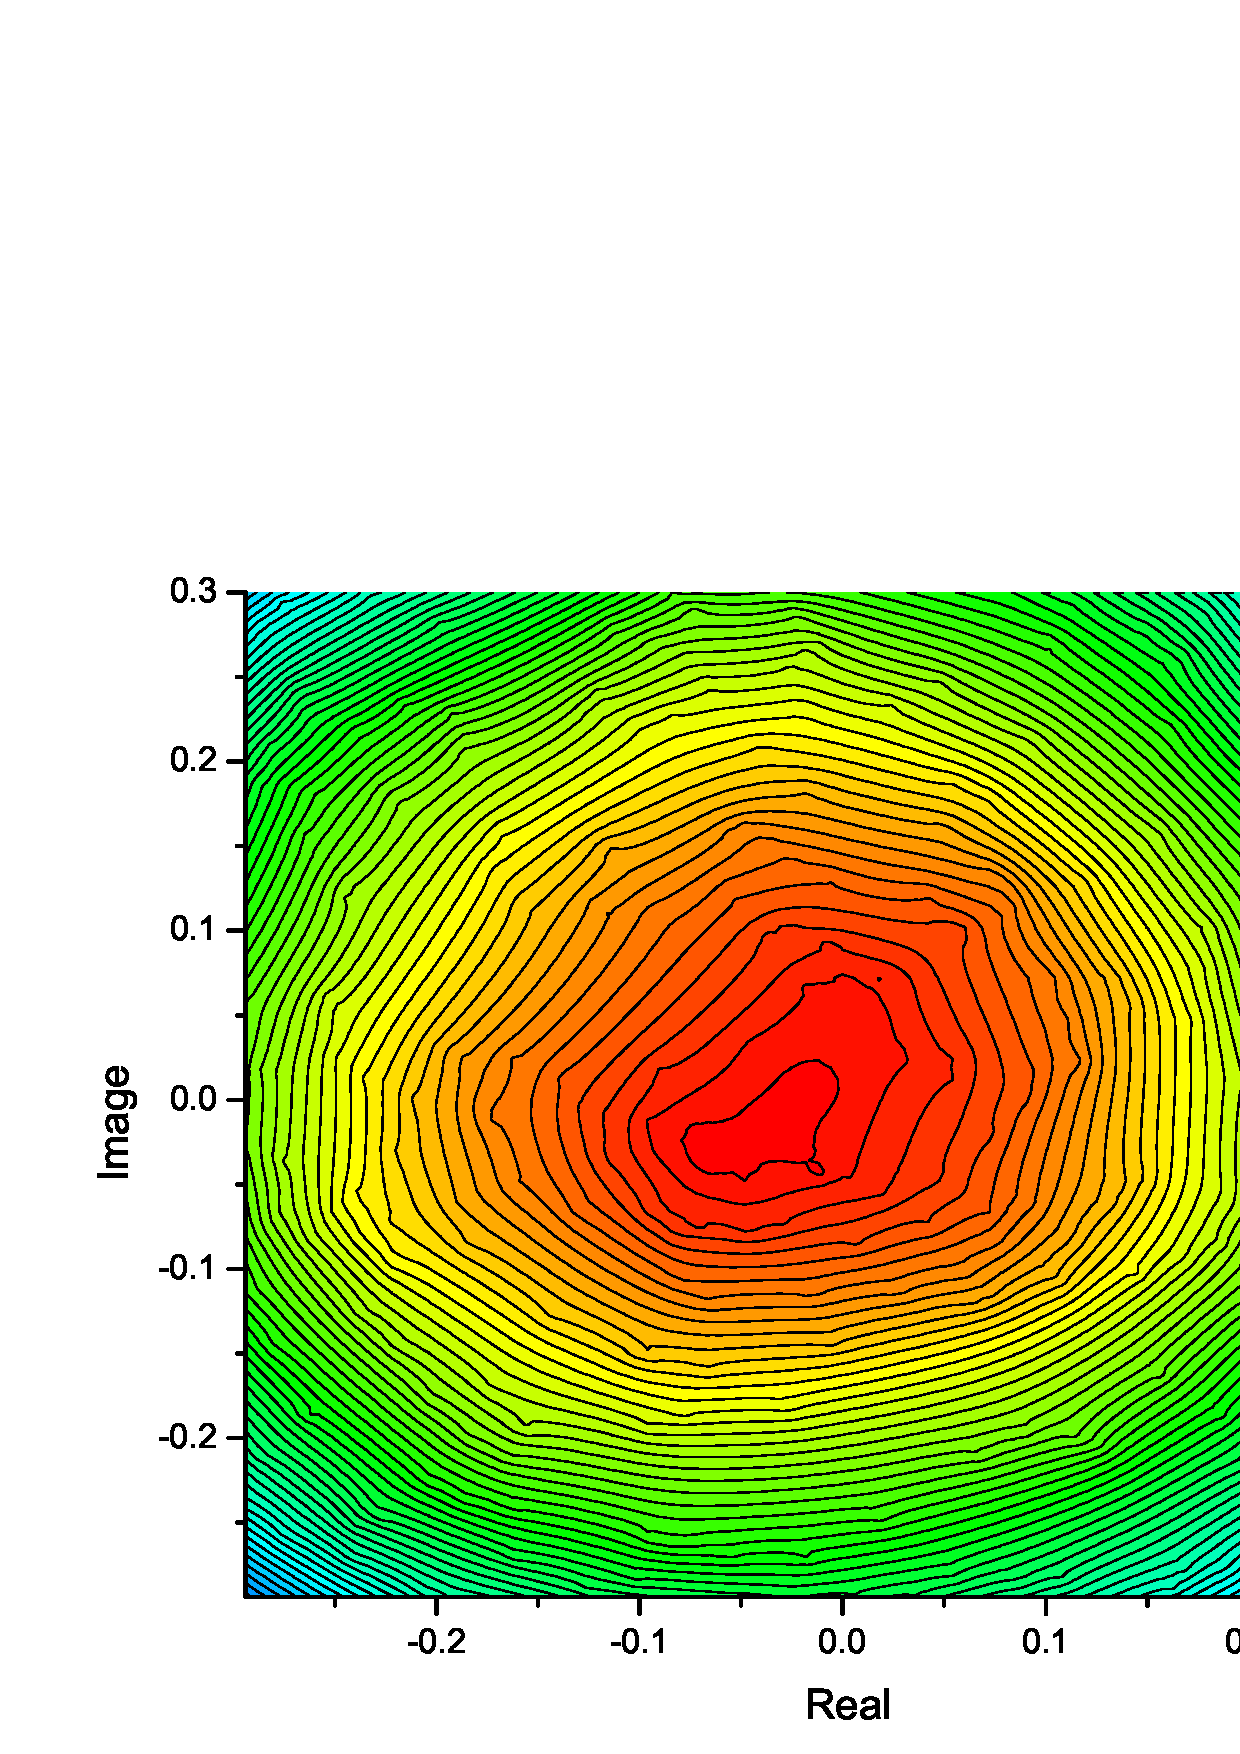
\includegraphics[scale=0.6]{gamma}


\part*{4.Result of $\gamma$ calculation}

To recover the true $\gamma$ we need to obtain the $\gamma$leads
to the largest likelihood.Since $\Delta\gamma=|\gamma-\gamma_{true}|$does
not depend on specific value of $\gamma_{true}$

only the value of $\Delta\gamma$ is recorded in the code.

The table below lists the mean value of |$\gamma-\gamma_{true}|$
for different Sample number N. The average is made over 6 tests.

\begin{tabular}{|c|c|c|c|}
\hline 
N & 200 & 1000 & 2000\tabularnewline
\hline 
\hline 
$\overline{|\Delta\gamma|}$ & 0.14 & 0.04 & 0.03\tabularnewline
\hline 
\end{tabular}
\end{document}
